\documentclass[12pt,a4paper,twoside,openright]{book}
\usepackage{lmodern}
\usepackage{amssymb,amsmath}
\usepackage{ifxetex,ifluatex}
\usepackage{fixltx2e} % provides \textsubscript
\ifnum 0\ifxetex 1\fi\ifluatex 1\fi=0 % if pdftex
  \usepackage[T1]{fontenc}
  \usepackage[utf8]{inputenc}
\else % if luatex or xelatex
  \ifxetex
    \usepackage{mathspec}
    \usepackage{xltxtra,xunicode}
  \else
    \usepackage{fontspec}
  \fi
  \defaultfontfeatures{Mapping=tex-text,Scale=MatchLowercase}
  \newcommand{\euro}{€}
\fi
% use upquote if available, for straight quotes in verbatim environments
\IfFileExists{upquote.sty}{\usepackage{upquote}}{}
% use microtype if available
\IfFileExists{microtype.sty}{%
\usepackage{microtype}
\UseMicrotypeSet[protrusion]{basicmath} % disable protrusion for tt fonts
}{}
\ifxetex
  \usepackage[setpagesize=false, % page size defined by xetex
              unicode=false, % unicode breaks when used with xetex
              xetex]{hyperref}
\else
  \usepackage[unicode=true]{hyperref}
\fi
\hypersetup{breaklinks=true,
            bookmarks=true,
            pdfauthor={},
            pdftitle={},
            colorlinks=true,
            citecolor=blue,
            urlcolor=blue,
            linkcolor=magenta,
            pdfborder={0 0 0}}
\urlstyle{same}  % don't use monospace font for urls
\usepackage{graphicx,grffile}
\makeatletter
\def\maxwidth{\ifdim\Gin@nat@width>\linewidth\linewidth\else\Gin@nat@width\fi}
\def\maxheight{\ifdim\Gin@nat@height>\textheight\textheight\else\Gin@nat@height\fi}
\makeatother
% Scale images if necessary, so that they will not overflow the page
% margins by default, and it is still possible to overwrite the defaults
% using explicit options in \includegraphics[width, height, ...]{}
\setkeys{Gin}{width=\maxwidth,height=\maxheight,keepaspectratio}
\setlength{\parindent}{0pt}
\setlength{\parskip}{6pt plus 2pt minus 1pt}
\setlength{\emergencystretch}{3em}  % prevent overfull lines
\providecommand{\tightlist}{%
  \setlength{\itemsep}{0pt}\setlength{\parskip}{0pt}}
\setcounter{secnumdepth}{0}

\date{}
% Table of contents formatting
\renewcommand{\contentsname}{Table des matières}
\setcounter{tocdepth}{3}
\setcounter{secnumdepth}{3}

\renewcommand*\listfigurename{Liste des figures}
\renewcommand*\listtablename{Liste des tableaux}

% Headers and page numbering
\usepackage{fancyhdr}
\pagestyle{plain}

% Fonts and typesetting
\setmainfont{TeX Gyre Pagella}
\setsansfont{Verdana}

% Set figure legends and captions to be smaller sized sans serif font
\usepackage[font={footnotesize,sf}]{caption}

\usepackage{siunitx}
\usepackage{float}
\usepackage{pdfpages}

% Adjust spacing between lines to 1.5
\usepackage{setspace}
\onehalfspacing
\raggedbottom

% Set margins
\usepackage[top=1.25in,bottom=1.25in]{geometry}

% Chapter styling
\usepackage[grey]{quotchap}
\makeatletter
\renewcommand*{\chapnumfont}{%
  \usefont{T1}{\@defaultcnfont}{b}{n}\fontsize{80}{100}\selectfont% Default: 100/130
  \color{chaptergrey}%
}
\makeatother

% Set colour of links to black so that they don't show up when printed
\usepackage{hyperref}
\hypersetup{colorlinks=true, linkcolor=black}

% Tables
\usepackage{booktabs}
\usepackage{threeparttable}
\usepackage{array}
\newcolumntype{x}[1]{>{\centering\arraybackslash}m{#1}}

\setlength{\parindent}{0.3cm} % Default is 15pt.

% Allow for long captions and float captions on opposite page of figures
\usepackage[rightFloats, CaptionBefore]{templates/packages/fltpage}

% Don't let floats cross subsections
\usepackage[section,subsection]{templates/packages/extraplaceins}

% University of Toulouse cover page package
\usepackage[emptypageafter, Ets=UT3]{templates/packages/tlsflyleaf/tlsflyleaf}

%% Titre, auteur, date, laboratoire, cotutelle
\title{Analyse et Modélisation de la Dynamique des Chromosomes durant la Mitose chez la Levure à Fission}
\author{Hadrien Mary}
\defencedate{16/12/2015}
\lab{Laboratoire de Biologie Cellulaire et Moléculaire du Contrôle de la Prolifération (UMR 5088)}
\docschool{École Doctorale Biologie Santé Biotechnologies}

%% Directeur(s) de thèse
\nboss{2}
\makesomeone{boss}{2}{Yannick Gachet}{}{}
\makesomeone{boss}{1}{Sylvie Tournier}{}{}
%% Referee
\nreferee{3}
\makesomeone{referee}{1}{Andrea Parmeggiani}{}{}
\makesomeone{referee}{2}{Benoit Arcangioli}{}{}
\makesomeone{referee}{3}{François Molino}{}{}

%% Jury
\njudge{7}
\makesomeone{judge}{1}{Kerstin Bystricky}{Professeur d'Université}{Président du Jury}
\makesomeone{judge}{2}{Andrea Parmeggiani}{Directeur de Recherche}{Membre du Jury}
\makesomeone{judge}{3}{Benoit Arcangioli}{Professeur d'Université}{Membre du Jury}
\makesomeone{judge}{4}{François Molino}{Maître de Conférences}{Membre du Jury}
\makesomeone{judge}{5}{Yannick Gachet}{Directeur de Recherche}{Membre du Jury}
\makesomeone{judge}{6}{Sylvie Tournier}{Directeur de Recherche}{Membre du Jury Invité}
\makesomeone{judge}{7}{Guillaume Gay}{Chercheur Indépendant}{Membre du Jury Invité}

% Redefines (sub)paragraphs to behave more like sections
\ifx\paragraph\undefined\else
\let\oldparagraph\paragraph
\renewcommand{\paragraph}[1]{\oldparagraph{#1}\mbox{}}
\fi
\ifx\subparagraph\undefined\else
\let\oldsubparagraph\subparagraph
\renewcommand{\subparagraph}[1]{\oldsubparagraph{#1}\mbox{}}
\fi

\begin{document}

\makeflyleaf

\newpage

\thispagestyle{empty}

\vspace*{\fill}

\begin{quote}
    {\centerline {\itshape « The dream of every cell is to become two cells. »}}
    \centerline{François Jacob, 1974}
  \end{quote}\vspace*{\fill}

\newpage

\thispagestyle{empty}

\frontmatter

\chapter{Résumé}\label{ruxe9sumuxe9}

La mitose est une étape clé du cycle cellulaire, très préservée chez
toutes les cellules eucaryotes, durant laquelle le matériel génétique de
la cellule (les chromosomes) est séparé en deux puis réparti de manière
égale dans les deux cellules filles. Cette équipartition du matériel
génétique est crucialle pour le maintien de la stabilité génétique.
Durant ce processus, la cellule forme une plaque métaphasique au centre
du fuseau mitotique composé des chromatides sœurs. Chaque chromatide est
alors attachée à son pôle respectif (on parle d'attachement bipolaire)
vers lequel elle se dirigera durant l'anaphase.

Les chromatides sont l'unité indivisible du matériel génétique durant la
mitose, à l'image des atomes dans une molécule. Initialement chacun de
ces « objets » est libre (non attaché) et positionné de manière non
ordonné dans le noyau. Toute la compléxité de la mitose est d'attacher
chacune des chromatides au bon pôle afin d'exercer des forces sur ces
derniers pour les positionner sur la plaque métaphasique au centre du
fuseau avant leur séparation et migration vers les pôles durant
l'anaphase.

Cette étape de la divison cellulaire requiert donc non seulement un
complexe réseau d'intéraction et de signalisation métabolique comme dans
beaucoup d'autre processus biologiques mais aussi un fin contrôle
spatio-temporel du mouvement et du positionnement des ces objets de
grande taille à l'echelle de la cellule: les chromatides.

Il est à ce jour clairement établi qu'une grande partie de l'énergie
nécessaire au mouvement des chromatides durant la mitose provient de la
dépolymérisation de l'extrémité + des microtubules (MTs) qui attache
chaque chromatide par l'intermédiaire d'un grand complexe protéique
appelé le kinétochore. Bien que le mécanisme de transfert d'énergie
entre la dépolymérisation des MTs et le mouvement des chromatides reste
encore très largement hypothétique.

La dynamique des chromosomes durant la mitose est par ailleurs largement
controlée par un grand nombre d'acteurs autres que les microtubules.
Certains d'entre eux étant responsables de l'attachement MTs-kinétochore
comme les complexes NDC80 et DAM1, tandis que d'autres sont impliqués
dans la régulation de la dynamique des microtubules comme la kinésine-8
et la kinésine-13 ainsi que différentes protéines associées aux
microtubules (MAPs) tel que XMAP215 ou encore EB1. De plus il existe des
preuves que les chromatides peuvent être transportées le long du fuseau
à l'aide de kinésine comme Cenp-E mais aussi de la dynéine.

Durant mon travail de thèse j'ai étudié la dynamique des chromosomes en
mitose chez la levure à fission qui à l'avantage de conserver les
mécanismes primordiaux de la mitose avec les eucaryotes supèrieurs. Deux
mécanismes que l'on retrouve chez de nombreuses cellules sont
l'alignement des chromosomes durant la métaphase ainsi qu'un mouvement
de va et vient plus ou moins régulier le long du fuseau aussi appelé
oscillations des chromosomes. J'ai montré en analysant les trajectoires
des chromosomes que ces deux processus sont pour une large part
indépendants chez la levure à fission (article en cours de révision). De
plus le processus d'alignement des chromosomes, encore mal compris, est
en parti contrôlé par la kinésine-8 via une activité dépendante de la
longueur des microtubules. Il semblerait donc qu'une protéine, la
kinésine-8, soit capable de fournir une information spatiale le long du
fuseau mitotique afin de positionner correctement les chromosomes. Enfin
j'ai utilisé un modèle mathématique du fuseau mitotique développé dans
l'équipe afin de tester de manière quantitative les hypothèses de
mécanisme du centrage des chromosomes par la kinésine-8.

L'ensemble de mon travail s'est donc intéressé au contrôle du mouvement,
de l'attachement et du positionnement des chromosomes durant la mitose
afin de mieux comprendre la biophysique du fuseau mitotique.

\chapter{Summary}\label{summary}

Mitosis is a critical step during cell cycle, well conserved in all
eukaryotic cells, during

Mitosis is a highly preserved process in all eukaryotic cells during
which genetic material (chromosomes) is divided in two parts and then
spread in both daughter cells. This equipartition is crucial for
maintaining genetic stability. During this process

(TODO: A FINIR)

\chapter{Remerciements}\label{remerciements}

\ldots{}

\tableofcontents

\setcounter{page}{1} \pagenumbering{arabic}

\mainmatter

\chapter{Introduction}\label{introduction}

La cellule est un objet complexe que l'Homme, depuis longtemps
maintenant, essaie de comprendre. En effet c'est en 1665 que Robert
Hooke, un savant anglais, observa pour la première fois au microscope
des «petites unités structurelles» qu'il décrira plus tard dans un
ouvrage intitulé «Micrographia» (Hooke (2003)). Sans vraiment réaliser
la portée de son observation, il venait de décrouvrir la cellule.

Plus tard, au début du 19ème siècle, la théorie cellulaire apparait;
stipulant que tous les organismes sont formés de cellules. La cellule
devient alors la plus petite unité indivisible qui compose le vivant.

Au milieu du 19ème siècle, un médecin allemand nommé Rudolf Virchow va
alors révolutionner la théorie cellulaire (Figure \ref{virchow}) en
démontrant qu'une cellule provient nécessairement qu'une autre cellule
(Virchow (1860)). Il écrivait alors \emph{«Omnis cellula e cellula»} qui
signifie «Toutes les cellules sont issues d'autres cellules.» Ses
travaux seront ensuite confirmés par un scientifique français du nom de
Louis Pasteur qui malgré de nombreuses controverses parvint à faire
tomber le mythe de la génération spontanée.

\begin{figure}[htbp]
\centering
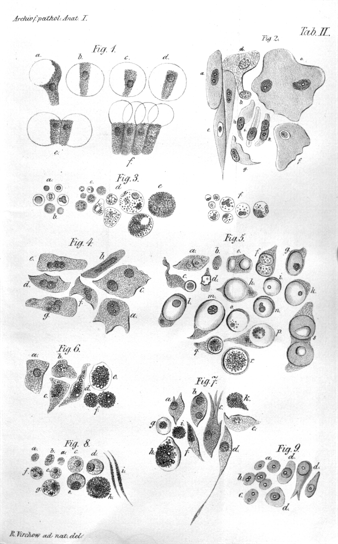
\includegraphics{figures/intro/virchow.jpg}
\caption{Illustration du livre «Cell theory» de Rudolf Virchow (Virchow,
1860)\label{virchow}}
\end{figure}

C'est véritablement au 20ème siècle que toute la complexité de la
cellule se dévoile grâce à l'apparition de nombreuses avancées
technologiques tel que la découverte de l'ADN, l'apparition de la
biologie moléculaire ainsi que la création de microscope toujours plus
précis.

Ce travail de thèse a pour objectif l'étude d'une phase tout à fait
cruciale durant la vie d'une cellule: le moment où elle se divise. Cette
étape, aussi appelé la mitose, permet selon le second axiome de la
théorie cellulaire, le maintien de l'intégrité cellulaire tout au long
des générations.

Enfin il est aussi bon de souligner que l'étude de la mitose est un
domaine d'étude important pour deux raisons majeures. Mieux comprendre
le fonctionnement du vivant par la compréhension de ce mécanisme
primordial sans lequel la vie ne serait jamais apparu sur Terre. Ainsi
que son rôle fondamentale dans l'étude du cancer; qui n'est autre qu'un
ensemble de maladie impliquant un déréglement de la divison cellulaire.
(TODO: A REFORMULER???)

\section{La vie d'une cellule}\label{la-vie-dune-cellule}

Le cycle cellulaire correspond à l'ensemble des étapes qui composent la
vie d'une cellule. Cette série d'évènement varie de manière considérable
d'une cellule à une autre. Le cycle cellulaire dépend de l'identité de
la cellule (principalement défini par son matèriel génétique) ainsi que
son contexte écologique; c'est à dire le milieu environnant dans lequel
elle se trouve.

Malgré son incroyable diversité, certaines étapes du cycle cellulaire
son communes à l'ensemble des cellules. La vie d'une cellule est composé
de deux étapes; une phase de croissance appelé l'interphase ainsi qu'une
phase de division appelé la mitose.

C'est durant l'interphase que la cellule va passer la plupart de sa vie
(Figure \ref{cycle}). Elle est composé de plusieurs étapes (Norbury and
Nurse (1992)):

\begin{itemize}
\item
  une étape de croissance (\textbf{phase G1}) durant laquelle la cellule
  va augmenter sa taille ainsi que son volume cellulaire. C'est aussi
  durant cette pèriode qu'elle va synthétisée un ensemble de protéine
  spécifique à son identité propre ainsi qu'au milieu dans lequel elle
  se trouve.
\item
  une étape de synthèse (\textbf{phase S}) durant laquelle la cellule va
  répliquer son matériel génétique, l'ADN. La duplication des
  chromosomes est une étape crucial pour le maintien de la stabilité
  génétique. En effet chacun des nucléotides (allant de quelques
  milliers à plusieurs milliard selon le type de cellule) doit être
  dupliqués avec une grande précision afin que les deux cellules filles
  se voit transmettre la même information génétique.
\item
  une étape de préparation de la division cellulaire (\textbf{phase G2})
  durant laquelle la cellule relance la synthèse de protéine et croit
  rapidement afin de préparer sa division. Cette phase est importante
  car elle possède un système de blocage du cycle cellulaire (aussi
  appelé «checkpoint» ou «point de contrôle») qui permet de retarder
  l'entrée en mitose en cas de problème de réplication de l'ADN apparu
  en phase S.
\end{itemize}

\begin{figure}[htbp]
\centering
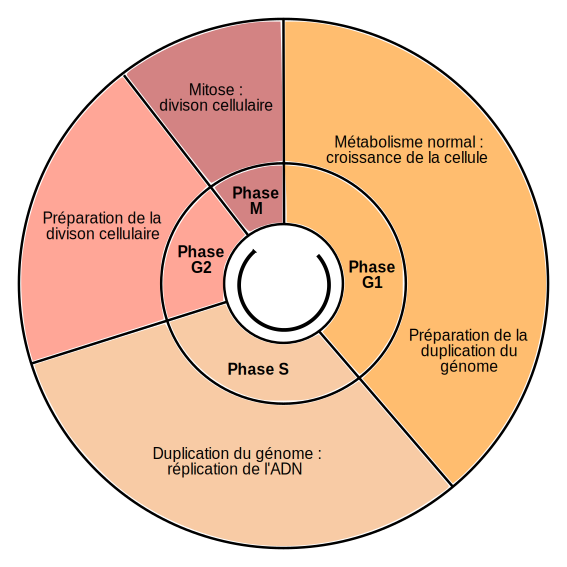
\includegraphics{figures/intro/cycle.png}
\caption{Les différentes étapes du cycle cellulaire \label{cycle}}
\end{figure}

Enfin la mitose qui fait suite à l'interphase (Figure \ref{cycle}) est
l'étape durant laquelle la cellule se divise en deux cellules filles.

Il est important d'insister sur le fait que dans la réalité, il existe
autant de cycle cellulaire différent qu'il existe de type de cellule. Il
est donc important de noter que malgré la conservation de certains
mécanismes primordiaux, chaque type de cellule possède son propre cycle
cellulaire (Lodish et al., 2000; Norbury and Nurse, 1992).

On soulignera aussi que l'un des enjeux de la biologie cellulaire
aujourd'hui est de comprendre quelle part de ces mécanismes sont
conservés entre différents type cellulaire et quelle part sont
spécifiques. (TODO A REFORMULER???)

\section{La mitose : une étape du cycle
cellulaire}\label{la-mitose-une-uxe9tape-du-cycle-cellulaire}

La dernière étape du cycle cellulaire est la mitose. Durant cette étape
la cellule mêre va se diviser en deux cellules filles. Tout les
mécanismes précédent et ceux composant la mitose ont pour objectif
d'assurer une division intègre et égale entre les deux cellules filles.

L'entrée en mitose est un événement contrôlé en grande parti par la
kinase Cdc2 aussi appelé Cdk1 (Nasmyth and Reed, 1980; Nurse and
Thuriaux, 1980). Cette protéine, conservé de la levure à l'Homme,
s'associe avec une protéine régulatrice, la Cycline B. Le complexe
s'active alors de manière transitoire pour former le fuseau mitotique.

\subsection{Les phases de la mitose}\label{les-phases-de-la-mitose}

De manière étonnante, la mitose est un processus relativement bien
conservé chez la majorité des cellules eucaryotes. Les grandes phases la
composant peuvent donc être décrites de manière commune pour un grand
nombre d'organismes.

Les différentes phases de la mitose sont (Figure \ref{mitosis}) :

\begin{itemize}
\item
  \textbf{prophase} : les brins d'ADN (la chromatine) se condensent pour
  former des structures ordonnées et séparées les unes des autres; les
  chromosomes. Les deux pôles (appelé centrosome chez les eucaryotes
  supèrieurs) se séparent et commencent à migrer vers leurs extrémités
  respectives afin de former le fuseau mitotique.
\item
  \textbf{prométaphase} : la membrane nucléaire se désassemble dans le
  cas d'une mitose ouverte (Boettcher and Barral (2013)) tandis qu'elle
  reste intact dans les mitoses fermées (répandu chez les protistes et
  organismes unicellulaires). Les chromosomes s'attachent aux
  microtubules par l'intermédiaire d'une structure protéique qui
  s'assemble au même moment au niveau du centromère des chromosomes: le
  kinétochore.
\item
  \textbf{métaphase} : les chromosomes alors attachés aux pôles par
  l'intermédiaire des microtubules viennent alors se positionner à
  l'équateur de la cellule pour former la plaque métaphasique. Cette
  étape cruciale de la mitose possède des mécanismes de détections des
  chromosomes mal attachés afin de retarder le passage à l'étape
  suivante si besoin.
\end{itemize}

La transition métaphase/anaphase possède un point de contrôle appelé le
SAC (Spindle Assembly Checkpoint) qui permet à la cellule d'arréter la
mitose en cas d'attachement incorrect (Musacchio and Salmon (2007)).
L'anaphase commence au moment où le complexe Cdc2-Cyclin B s'inactive
par l'activation de l'APC (Anaphase Promoting Complex). L'APC est une
ubiquitin ligase capable de dégradé la Cyclin B (Sivakumar and Gorbsky
(2015)).

\begin{itemize}
\item
  \textbf{anaphase} : durant l'anaphase A, le complexe cohésine reliant
  les chromatides soeurs est dabord dégradé (Oliveira et al. (2010)).
  Ensuite chaque chromatide est «tiré» vers son pôle respectif par la
  dépolymérisation des microtubules qui les attachent tandis que durant
  l'anaphase B, le fuseau mitotique s'allonge, éloignant alors les pôles
  et les chromosomes loin du centre de la cellule. On notera que ces
  deux phases peuvent être distinctes ou pas selon le type de cellule
  étudié.
\item
  \textbf{télophase} : les microtubules attachant les kinétochores se
  désagrègent, les chromosomes se décondensent retournant à leurs états
  initials de brins d'ADN. L'enveloppe nucléaire se reforme dans le cas
  d'une mitose ouverte.
\item
  \textbf{cytokinèse} : à ce stade, la mitose est fini. Durant cette
  période, la cellule se divise grâce à la formation d'un sillon au
  niveau de la membrane cytoplasmique qui va alors s'invaginer jusqu'à
  «couper» la cellule mêre en deux cellules filles.
\end{itemize}

\begin{figure}[htbp]
\centering
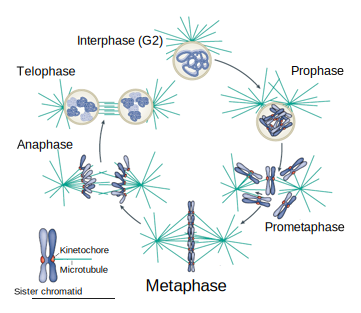
\includegraphics{figures/intro/mitosis.png}
\caption{Les différentes étapes de la mitose (adapté de Cheeseman and
Desai (2008)) \label{mitosis}}
\end{figure}

\subsection{Le kinétochore}\label{le-kinuxe9tochore}

Le kinétochore est

\begin{figure}[htbp]
\centering
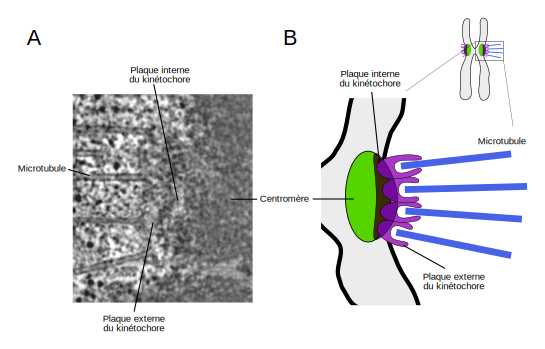
\includegraphics{figures/intro/kt.png}
\caption{A. Vu d'un kinétochore humain de côté par microscopie
électronique (Cheeseman and Desai (2008)). B. Schéma des différentes
plaques d'un kinétochore. \label{kt}}
\end{figure}

\begin{figure}[htbp]
\centering
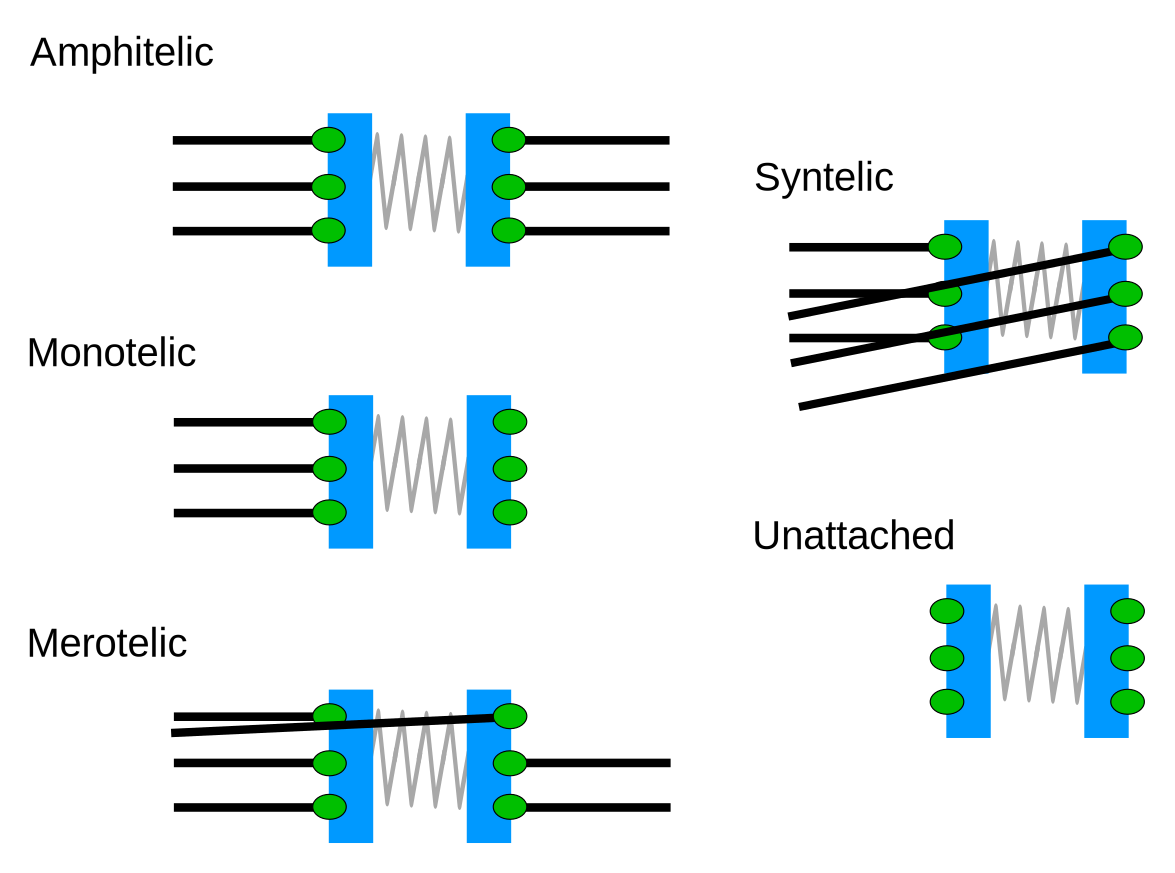
\includegraphics{figures/intro/attachments.png}
\caption{Les différents type d'attachments des chromosomes aux
microtubules}
\end{figure}

\section{L'appareil mitotique : un objet sous
contrainte}\label{lappareil-mitotique-un-objet-sous-contrainte}

\section{La métaphase : point d'orgue de la division
cellulaire}\label{la-muxe9taphase-point-dorgue-de-la-division-cellulaire}

\section{La dynamique des chromosomes durant la
métaphase}\label{la-dynamique-des-chromosomes-durant-la-muxe9taphase}

\section{Modélisation mathématique du mouvement des chromosomes en
mitose}\label{moduxe9lisation-mathuxe9matique-du-mouvement-des-chromosomes-en-mitose}

\section{La levure à fission : un organisme modéle pour l'étude du cycle
cellulaire}\label{la-levure-uxe0-fission-un-organisme-moduxe9le-pour-luxe9tude-du-cycle-cellulaire}

\section{Problématique}\label{probluxe9matique}

\chapter{Résultats}\label{ruxe9sultats}

\section{« Fission yeast Kinesin-8 controls chromosome congression
independently of oscillations
»}\label{fission-yeast-kinesin-8-controls-chromosome-congression-independently-of-oscillations}

\includepdf[pages=-,scale=10]{text/4_resultats/mwe.pdf}

\section{Modélisation bio-mécanique du fuseau
mitotique}\label{moduxe9lisation-bio-muxe9canique-du-fuseau-mitotique}

\begin{itemize}
\tightlist
\item
  parler modéle d'attachement à deux états et des avantages d'un modèle
  à trois états
\end{itemize}

\section{Analyse du mouvement des chromosomes par la MSD via une
approche
bayésienne}\label{analyse-du-mouvement-des-chromosomes-par-la-msd-via-une-approche-bayuxe9sienne}

\begin{itemize}
\tightlist
\item
  bla bla bla
\end{itemize}

\chapter{Discussion}\label{discussion}

\section{Le mouvement de chromosomes durant la
mitose}\label{le-mouvement-de-chromosomes-durant-la-mitose}

\section{\texorpdfstring{Le mécanisme d'alignement des chromosomes: de
l'\emph{in silico} à l'\emph{in
vivo}}{Le mécanisme d'alignement des chromosomes: de l'in silico à l'in vivo}}\label{le-muxe9canisme-dalignement-des-chromosomes-de-lin-silico-uxe0-lin-vivo}

\appendix

\chapter{Annexes}\label{annexes}

\section{Annexe 1 : bla bla bla bla}\label{annexe-1-bla-bla-bla-bla}

\backmatter

\chapter{Bibliographie}\label{bibliographie}

\bibliographystyle{plain}\bibliography{library}

Boettcher, B., and Barral, Y. (2013). The cell biology of open and
closed mitosis.Nucleus (Austin, Tex.)\emph{4}, 160--165.

Cheeseman, I.M., and Desai, A. (2008). Molecular architecture of the
kinetochore-microtubule interface.Nature Reviews. Molecular Cell
Biology\emph{9}, 33--46.

Hooke, R. (2003). Micrographia: Or Some Physiological Descriptions of
Minute Bodies Made by Magnifying Glasses, with Observations and
Inquiries Thereupon(Dover Publications).

Lodish, H., Berk, A., Zipursky, S.L., Matsudaira, P., Baltimore, D., and
Darnell, J. (2000). Overview of the Cell Cycle and Its Control(W. H.
Freeman).

Musacchio, A., and Salmon, E.D. (2007). The spindle-assembly checkpoint
in space and time.Nature Reviews. Molecular Cell Biology\emph{8},
379--393.

Nasmyth, K.A., and Reed, S.I. (1980). Isolation of genes by
complementation in yeast: molecular cloning of a cell-cycle
gene.Proceedings of the National Academy of Sciences\emph{77},
2119--2123.

Norbury, C., and Nurse, P. (1992). Animal cell cycles and their
control.Annual Review of Biochemistry\emph{61}, 441--470.

Nurse, P., and Thuriaux, P. (1980). REGULATORY GENES CONTROLLING MITOSIS
IN THE FISSION YEAST SCHIZOSACCHAROMYCES POMBE.Genetics\emph{96},
627--637.

Oliveira, R. a, Hamilton, R.S., Pauli, A., Davis, I., and Nasmyth, K.
(2010). Cohesin cleavage and Cdk inhibition trigger formation of
daughter nuclei.Nature Cell Biology\emph{12}, 185--192.

Sivakumar, S., and Gorbsky, G.J. (2015). Spatiotemporal regulation of
the anaphase-promoting complex in mitosis.Nature Publishing
Group\emph{16}, 82--94.

Virchow, R.L.K. (1860). Cellular pathology(John Churchill).

\end{document}
